\tikzset{every picture/.style={line width=0.75pt}} %set default line width to 0.75pt        

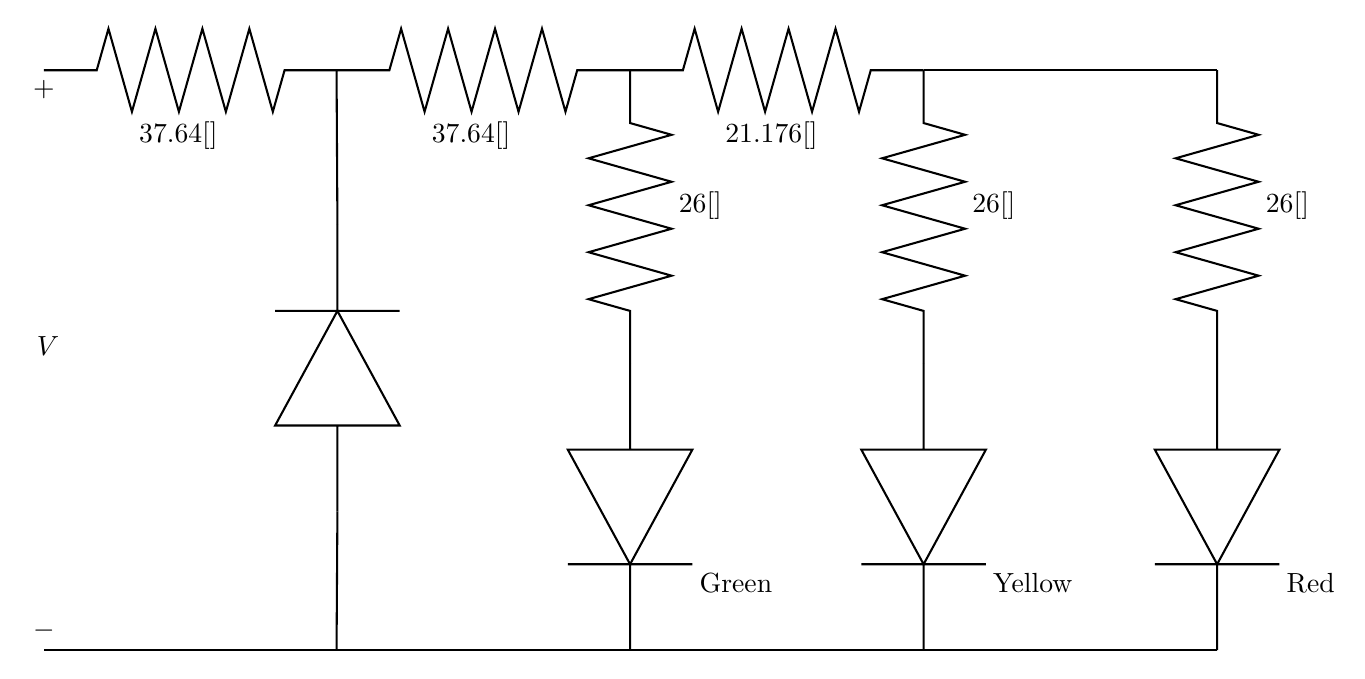
\begin{tikzpicture}[x=0.75pt,y=0.75pt,yscale=-1,xscale=1]
%uncomment if require: \path (0,757); %set diagram left start at 0, and has height of 757

%Shape: Diode [id:dp9916766022166023] 
\draw   (611,293.4) -- (581,348.6) -- (551,293.4) -- (611,293.4) -- cycle (581,252) -- (581,293.4) (611,348.6) -- (551,348.6) (581,348.6) -- (581,390) ;
%Shape: Diode [id:dp47724199606317685] 
\draw   (469.58,293.4) -- (439.58,348.6) -- (409.58,293.4) -- (469.58,293.4) -- cycle (439.58,252) -- (439.58,293.4) (469.58,348.6) -- (409.58,348.6) (439.58,348.6) -- (439.58,390) ;
%Straight Lines [id:da43394379079125567] 
\draw    (581,390) -- (439.58,390) ;
%Shape: Resistor [id:dp7260924477087448] 
\draw   (581,110.58) -- (581,136.03) -- (601,141.69) -- (561,153.01) -- (601,164.32) -- (561,175.63) -- (601,186.95) -- (561,198.26) -- (601,209.57) -- (561,220.89) -- (581,226.54) -- (581,252) ;
%Shape: Resistor [id:dp09973725738727013] 
\draw   (439.58,110.58) -- (439.58,136.03) -- (459.58,141.69) -- (419.58,153.01) -- (459.58,164.32) -- (419.58,175.63) -- (459.58,186.95) -- (419.58,198.26) -- (459.58,209.57) -- (419.58,220.89) -- (439.58,226.54) -- (439.58,252) ;
%Straight Lines [id:da9934104451259984] 
\draw    (581,110.58) -- (439.58,110.58) ;
%Shape: Resistor [id:dp5223648498783691] 
\draw   (298.16,110.58) -- (323.61,110.58) -- (329.27,90.58) -- (340.58,130.58) -- (351.9,90.58) -- (363.21,130.58) -- (374.52,90.58) -- (385.84,130.58) -- (397.15,90.58) -- (408.47,130.58) -- (414.12,110.58) -- (439.58,110.58) ;
%Shape: Diode [id:dp30609907031657446] 
\draw   (328.16,293.4) -- (298.16,348.6) -- (268.16,293.4) -- (328.16,293.4) -- cycle (298.16,252) -- (298.16,293.4) (328.16,348.6) -- (268.16,348.6) (298.16,348.6) -- (298.16,390) ;
%Shape: Resistor [id:dp3336013122238709] 
\draw   (298.16,110.58) -- (298.16,136.03) -- (318.16,141.69) -- (278.16,153.01) -- (318.16,164.32) -- (278.16,175.63) -- (318.16,186.95) -- (278.16,198.26) -- (318.16,209.57) -- (278.16,220.89) -- (298.16,226.54) -- (298.16,252) ;
%Straight Lines [id:da4142874846716025] 
\draw    (439.58,390) -- (298.16,390) ;
%Shape: Resistor [id:dp416533824669727] 
\draw   (156.74,110.58) -- (182.19,110.58) -- (187.85,90.58) -- (199.16,130.58) -- (210.48,90.58) -- (221.79,130.58) -- (233.1,90.58) -- (244.42,130.58) -- (255.73,90.58) -- (267.04,130.58) -- (272.7,110.58) -- (298.16,110.58) ;
%Straight Lines [id:da6359356780714503] 
\draw    (298.16,390) -- (156.74,390) ;
%Shape: Diode [id:dp6533823694560318] 
\draw   (127.16,281.74) -- (157.16,226.54) -- (187.16,281.74) -- (127.16,281.74) -- cycle (157.16,323.14) -- (157.16,281.74) (127.16,226.54) -- (187.16,226.54) (157.16,226.54) -- (157.16,185.14) ;
%Straight Lines [id:da919246511874256] 
\draw    (156.74,110.58) -- (157.16,185.14) ;
%Straight Lines [id:da15872631988300578] 
\draw    (157.16,323.14) -- (156.74,390) ;
%Shape: Resistor [id:dp9457923449115067] 
\draw   (15.74,110.58) -- (41.19,110.58) -- (46.85,90.58) -- (58.16,130.58) -- (69.48,90.58) -- (80.79,130.58) -- (92.1,90.58) -- (103.42,130.58) -- (114.73,90.58) -- (126.04,130.58) -- (131.7,110.58) -- (157.16,110.58) ;
%Straight Lines [id:da3465774446259271] 
\draw    (157.16,390) -- (15.74,390) ;

% Text Node
\draw (603,167.72) node [anchor=north west][inner sep=0.75pt]    {$26[ \si{\ohm}]$};
% Text Node
\draw (461.58,167.72) node [anchor=north west][inner sep=0.75pt]    {$26[ \si{\ohm}]$};
% Text Node
\draw (320.16,167.72) node [anchor=north west][inner sep=0.75pt]    {$26[ \si{\ohm}]$};
% Text Node
\draw (342.58,133.98) node [anchor=north west][inner sep=0.75pt]    {$21.176[ \si{\ohm}]$};
% Text Node
\draw (201.16,133.98) node [anchor=north west][inner sep=0.75pt]    {$37.64[ \si{\ohm}]$};
% Text Node
\draw (613,351.6) node [anchor=north west][inner sep=0.75pt]   [align=left] {Red};
% Text Node
\draw (471.58,351.6) node [anchor=north west][inner sep=0.75pt]   [align=left] {Yellow};
% Text Node
\draw (330.16,351.6) node [anchor=north west][inner sep=0.75pt]   [align=left] {Green};
% Text Node
\draw (15.74,113.98) node [anchor=north] [inner sep=0.75pt]    {$+$};
% Text Node
\draw (15.74,386.6) node [anchor=south] [inner sep=0.75pt]    {$-$};
% Text Node
\draw (17.74,243.29) node    {$V$};
% Text Node
\draw (60.16,133.98) node [anchor=north west][inner sep=0.75pt]    {$37.64[ \si{\ohm}]$};


\end{tikzpicture}
